\chapter{The Minimal Supersymmetric Model}
\label{chap:mssm}

In addition to the SU(3)$\times$SU(2)$\times$U(1) symmetry imposed on the Lagrangian within the Standard Model, one can introduce additional \textit{supersymmetrys} to the theory. Supersymmetry transformations act on fields containing both fermionic and bosonic degrees of freedom, the Lagrangian is required to remain invariant under rotations between these two states. Many such extensions to the Standard Model exist, but only the simplest of these, requiring a single global transformation $Q$ is phenomenologically viable: the Minimal Supersymmetric Standard Model (MSSM).

Within the MSSM, every SM particle has a \textit{superpartner} which differs by 1/2 unit of spin but otherwise has identical properties. For example, the electron is paired with an electrically charged, massive, spin-0 scalar field, called a ``selectron''. 


A striking prediction of the MSSM is more than a doubling of the known particle content of the Universe. 
In addition to the single SM Higgs doublet, the MSSM requires another spin-0 Higgs isospin doublet, with opposite hypercharge. These two spin-0 doublets each have their own chiral superpartner. Table \ref{tab:mssmparticles} lists the fields required within the MSSM (the sort of complement of Table \ref{tab:sm}). As the nature of the newly supersymmetric electroweak sector is unknown, the various components of the fields may mix. The charged components from the new SU(2) fields and the Higgs summarized in Table \ref{tab:mixing} (color charge prevents gluinos from mixing outside QCD). This chapter is adapted from \cite{susyprimer}.

\begin{table}[hb!]
\caption{Summary of the additional particle content within the MSSM.}
\label{tab:mssmparticles}
\centering
\begin{tabular}{c|ll}
\hline\hline
\textbf{SM Gauge Sector} & sfermions & gauginos \\
%\hdashline
\hline
SU(3) & $\tilde{u}, \tilde{d}, \tilde{c}, \tilde{s}, \tilde{t}, \tilde{b}$ & $\tilde{g}_{1...8}$ \\
\hline
& $\widetilde{Q}_{L}$ = $\begin{pmatrix} \tilde{u} \\ \tilde{d} \end{pmatrix}_{L}, \begin{pmatrix} \tilde{s} \\ \tilde{c} \end{pmatrix}_{L}, \begin{pmatrix} \tilde{t} \\ \tilde{b} \end{pmatrix}_{L} $ &  \\
SU(2) $\times$ U(1) & $\tilde{q} = \tilde{u}, \tilde{d}, \tilde{c}, \tilde{s}, \tilde{t}, \tilde{b}$ & $\widetilde{W}_{012}, \widetilde{B}_{0}$\\
& $\widetilde{L}_{L}$ = $\begin{pmatrix} \tilde{\nu}_{e} \\ \tilde{e}^{-} \end{pmatrix}_{L} , \begin{pmatrix} \tilde{\nu}_{\mu} \\ \tilde{\mu}^{-} \end{pmatrix}_{L} , \begin{pmatrix} \tilde{\nu}_{\tau} \\ \tilde{\tau}^{-}\end{pmatrix}_{L} $ & \\
& $\tilde{\ell} = (\tilde{e}, \tilde{\mu}, \tilde{\tau})$ & \\
\hline
& \multicolumn{1}{c}{spin-0} &  \multicolumn{1}{c}{spin-1/2} \\
\textbf{Higgs Sector} & $H_{u} = \begin{pmatrix} H_{u}^{+} \\ H_{u}^{0} \end{pmatrix},  H_{d} = \begin{pmatrix} H_{d}^{0} \\ H_{d}^{-} \end{pmatrix}$ & $\widetilde{H}_{u} = \begin{pmatrix} \widetilde{H}_{u}^{+} \\ \widetilde{H}_{u}^{0} \end{pmatrix},  \widetilde{H}_{d} = \begin{pmatrix} \widetilde{H}_{d}^{0} \\ \widetilde{H}_{d}^{-} \end{pmatrix}$\\
\hline\hline
\end{tabular}
\end{table}



\begin{table}[hb!]
\caption{Mixing of the supersymmetric electroweak fields.}
\centering
\begin{tabular*}{0.75\textwidth}{ll}
\hline
label 1 & label 2 \\
item 1  & item 2 \\
\hline
\end{tabular*}
\end{table}

Matter particles (both the left and right-chiral components seperately) are placed in \textit{chiral supermultiplets} consisting of a spin-1/2 Majorana fermion $\psi$ and complex scalar field $\phi$. In the massless and non-interacting case (i.e. just the two kinetic terms in the Lagrangian, known as the \textit{Wess-Zumino model} \cite{wesszumino}), the transformation laws of the fields can be deduced by demanding invariance under the simple Lagrangian, they are found to be:
 
\begin{equation}
\begin{array}{l}
\phi \xrightarrow[]{\text{Q}} \phi + \epsilon \psi \\
\psi \xrightarrow[]{\text{Q}} \psi - i ( \sigma^{\mu} \epsilon^{\dagger} ) \partial_{\mu} \phi \\
\end{array}
\end{equation}
where $\epsilon$ is a 2-component Weyl \textbf{spinor} parametrizing the transformation. For the duration of this chapter, all references to \textit{auxiliary} fields will be omitted. Auxiliary fields are internal to the theory and must be introduced to allow the fields to satisfy their classical wave equations.

The requirement of renormalizability restricts the numbers of fields in any interaction involving $\psi$ and $\phi$, the most generic Lagrangian for a chiral supermultiplet is of the form:

\begin{equation}
\label{eq:lchiral}
\mathcal{L}_{chiral} = - D^{\mu}\phi^{*}D{\mu}\phi - V(\phi, \phi^{*}) + i \psi^{\dagger}\bar{\sigma}^{\mu} D{\mu}\psi - \frac{1}{2} (M \psi \psi + h.c.) - \frac{1}{2} (y \phi  \psi \psi + h.c.)
\end{equation}

where $D^{\mu}$ is the covariant derivative, $V(\phi, \phi^{*})$ is a scalar potential for the theory, $\bar{\sigma}^{0}$ is the 2x2 identity matrix and $\bar{\sigma}^{123}\equiv-\sigma^{123}$, M is a (Majorana) mass term, $\psi\psi\equiv\epsilon^{ab}\psi_{a}\psi_{b}$, and $y$ is a Yukawa coupling. The Yukawa coupling connects two SM fermions with the corresponding supersymmetric scalar field - a vertex diagram for this process is seen in Figure \ref{fig:mssmfeyn}(a). The covariant derivative $\partial_{\mu} \phi \rightarrow \partial_{\mu}\phi -igA^{a}_{\mu}T^{a}\phi$, when introduced in the kinetic term, creates two interactions between the SM gauge bosons and the new supersymmetric scalar field: $-ig[(\partial_{\mu}\phi)A^{a}_{\mu}T^{a}\phi+h.c.]$ and $g^{2}A^{a\mu}\phi^{*}t^{a}A^{a}_{\mu}T^{a}\phi$, seen in Figures \ref{fig:mssmfeyn}(d) and (e), respectively. Throughout this chapter I will only discuss interactions involving at least one SM particle and at least one supersymmetric particle.

Gauge bosons (before spontaneous symmetry breaking) are placed in \textit{gauge supermultiplets} consisting of gauge bosons A$_{\mu}^{a}$ and spin-1/2 gauginos $\lambda^{a}$; $a$ is a label which runs over the SM gauge fields within the theory. Under the supersymmetry, fields can be found to transform as:

\begin{equation}
\begin{array}{l}
A_{\mu}^{a} \xrightarrow[]{\text{Q}} A_{\mu}^{a} - \frac{1}{\sqrt{2}} ( \epsilon^{\dagger} \bar{\sigma}_{\mu} \lambda + h.c)\\
\lambda_{\alpha}^{a} \xrightarrow[]{\text{Q}} \lambda_{\alpha} + \frac{i}{2\sqrt{2}}(\sigma^{\mu}\bar{\sigma}^{\nu}\epsilon)F_{\mu\nu}^{a}
\end{array}
\end{equation}

where $F_{\mu\nu}^{a}$ is the regular field strength tensor for the gauge field $A_{\mu}^{a}$. The SM symmetries (i.e. SU(3), SU(2), U(1)) transform the gauge supermultiplet in the following way:

\begin{equation}
\begin{array}{l}
A_{\mu}^{a} \xrightarrow[]{\text{SM}}  A_{\mu}^{a} + \partial_{\mu}\Lambda^{a} + gf^{ijk}A_{\mu}^{b}\Lambda^{c}\\
\lambda^{a} \xrightarrow[]{\text{SM}}  \lambda^{a} + gf^{abc}\lambda^{b}\Lambda^{c}
\end{array}
\end{equation}
where $\Lambda^{a}$ is a parameter describing the the transformation. (The transformation law for $A^{\mu}$ is the same we have seen in Chapter \ref{chap:sm}.)

The Lagrangian for a free gauge multiplet consists simply of the kinetic terms for each field $A_{\mu}^{a}$ and $\lambda^{a}$:
\begin{equation}
\mathcal{L}_{gauge} = -\frac{1}{4}F_{\mu\nu}F^{\mu\nu} + i \lambda^{\dagger}\bar{\sigma}^{\mu}\nabla\lambda^{a}
\end{equation}
where $f^{abc}$ are the structure constants of the gauge group. $\nabla\lambda^{a} = \partial_{\mu}\lambda^{a}+gf^{abc}A^{b}_{\mu}\lambda^{c}$ represents the covariant derivative acting on $\lambda^{a}$ - creating an interaction term between a gauge boson and two gauginos: $i g \lambda^{\dagger}\bar{\sigma}^{\mu} f^{abc}A^{b}_{\mu}\lambda^{c}$, as seen in Figure \ref{fig:mssmfeyn}c.

The requirement of renormalization restricts the interactions between the gauge and chiral supermultiplets to be only of the form $-\sqrt{2}g(\phi^{*}T^{a}\psi\lambda^{a}+h.c.)$, involving a single spin-0, spin-1/2, and spin-1 particle - a vertex diagram is seen in Figure \ref{fig:mssmfeyn}(e).

\begin{figure}[hb!]
\centering
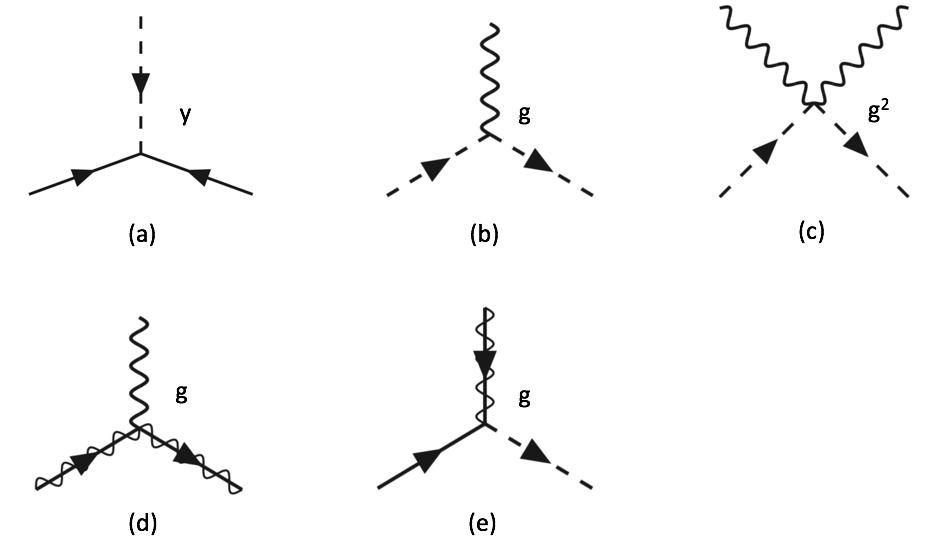
\includegraphics[width=0.7\textwidth]{figs/mssmfeyn.png}
\caption{Interactions between SM and MSSM particles. $y$ is a Yukawa coupling to be determined, $g$ is the SM gauge coupling.}
\label{fig:mssmfeyn}
\end{figure}

Within a supersymmetric theory, the superpartners are required to have the same mass as their corresponding SM field. If SUSY were exact, we would have expected to see evidence of sparticles over the years. There must be some mechanism which generates large mass for the sparticles such that their production is highly suppressed at our colliders. The remainder of this thesis presents a search for evidence of physics beyond the SM, such as the MSSM. Our motivation is taken from final state topologies arising from gluino pair production - possible mechanisms seen in Figure \ref{fig:gluinopair}. The gluino is the spin-1/2 fermion which is the superpartner to the gluon, the mediator of the strong force. Within the context of QCD - the chiral supermultiplets consist of spin-1/2 quarks and spin-0 squarks. Searches for supersymmetric particles of QCD are partly motivated by the fact that most of their production mechanisms proceed through diagrams proportional to the strong coupling constant $g_{s}$, which is largest among the three in the SM. The supersymmetric partners of QCD necessarily carry color charge, and therefore the QCD squarks and gluinos do not directly interact with other MSSM particles. There have been many searches for SUSY which provide lower limits on the mass of the gluino, such as \cite{CMS-SUS-16-033} or \cite{CMS-SUS-15-002}, and its current limit is at about 2 TeV. Figure \ref{fig:oldlimits} summarizes the results of one of these searches, excluding gluinos below 1.8 TeV given assumptions about the decay (seen in the diagram below the plot). The blob in the diagrams below the limit plots indicates we are not interested in the particular production mechanism, but in the decay chain.

\begin{figure}[hb!]
\centering
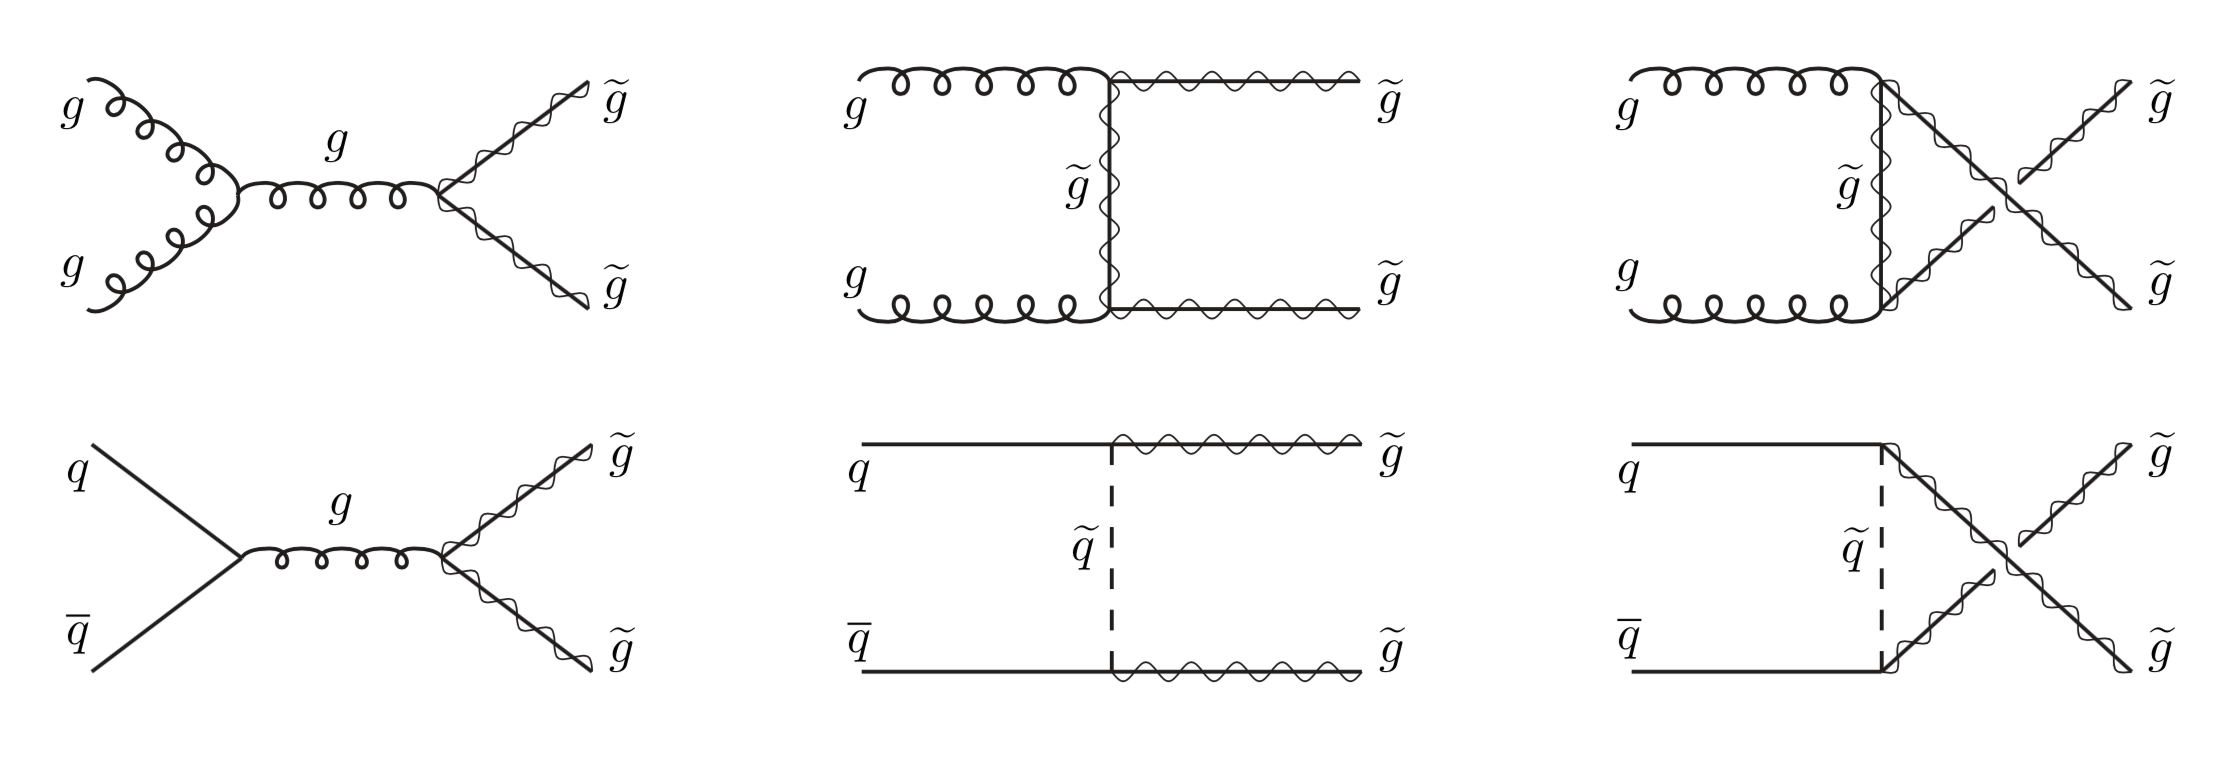
\includegraphics[width=0.9\textwidth]{figs/gluinopair}
\caption{Tree-level gluino pair-production mechanisms.}
\label{fig:gluinopair}
\end{figure}

\begin{figure}[hb!]
\centering
\begin{subfigure}{0.4\textwidth}
\centering
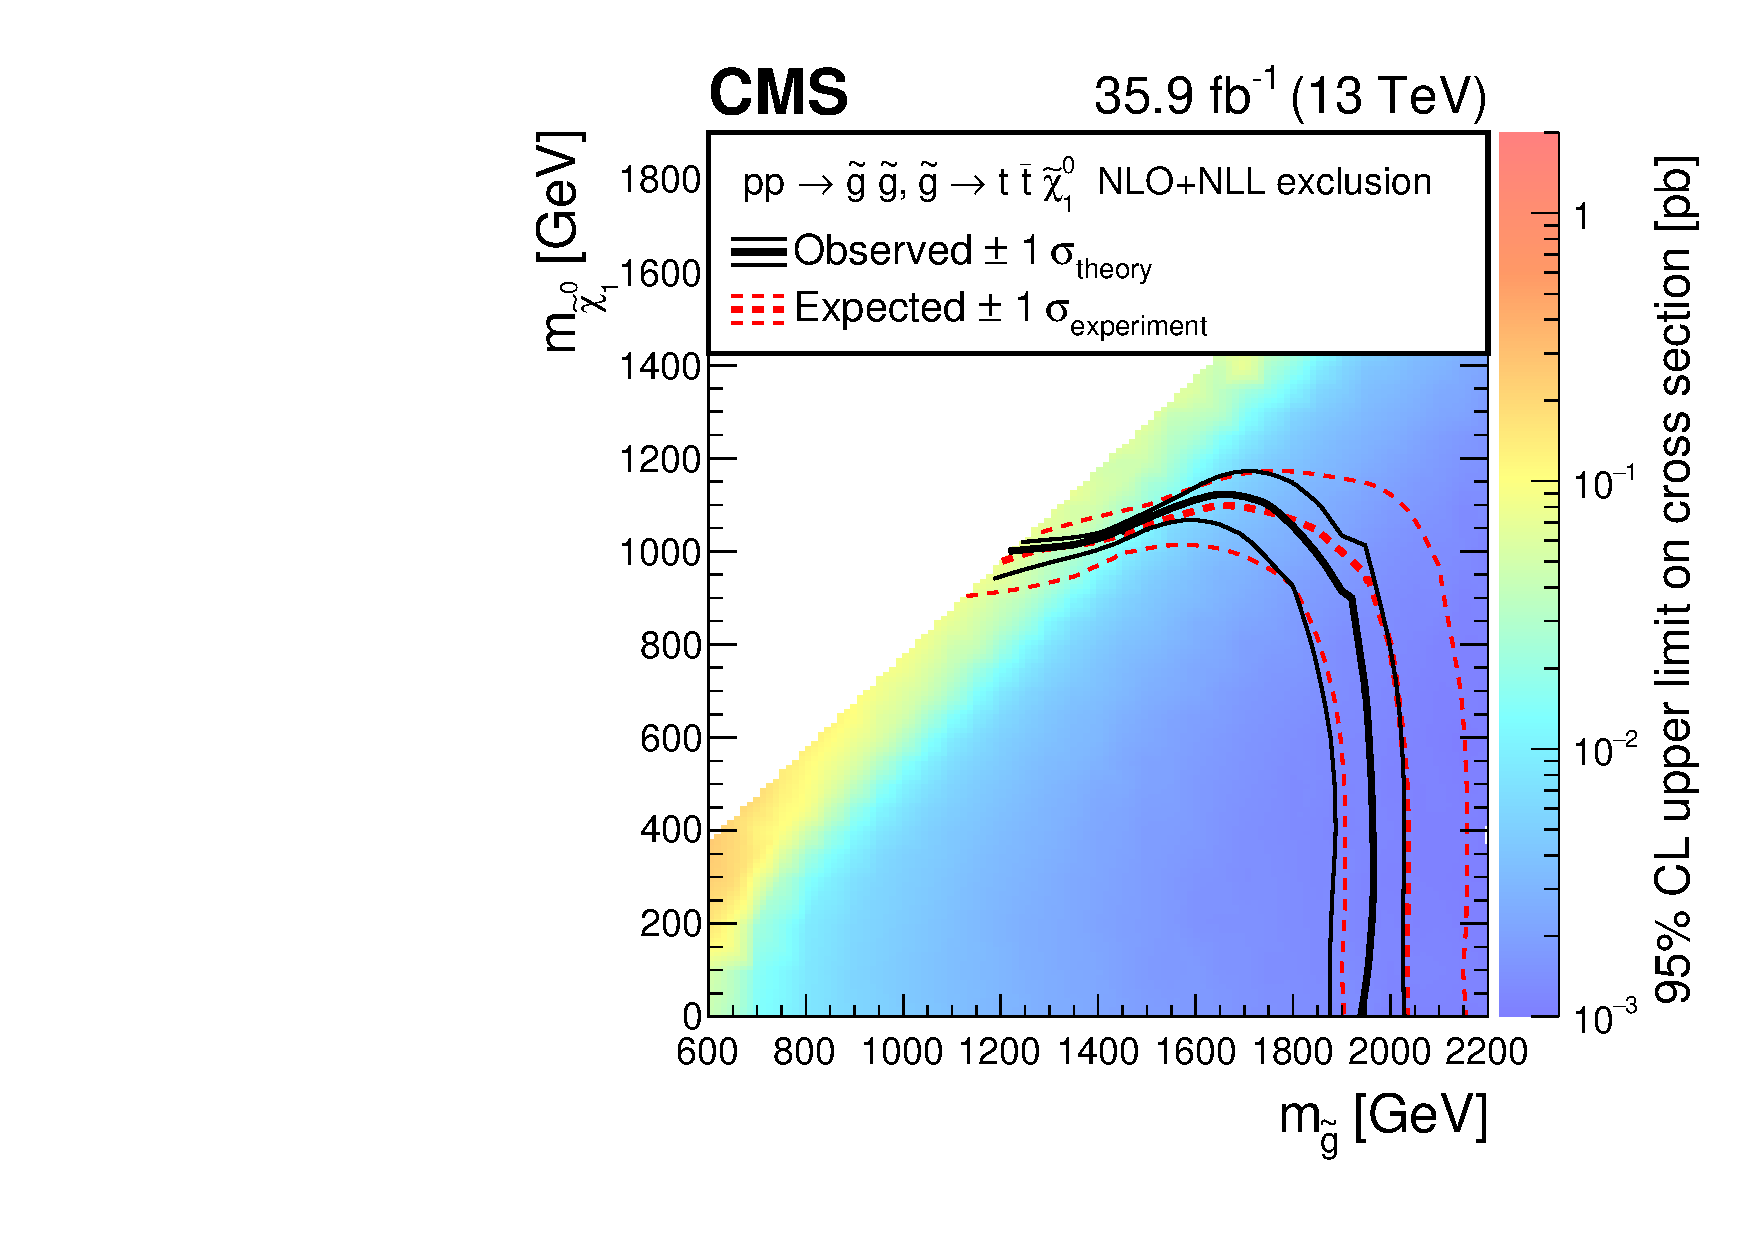
\includegraphics[width=\textwidth]{figs/CMS-SUS-16-033_Figure_012-a.pdf}  
\end{subfigure}
\begin{subfigure}{0.4\textwidth}
\centering
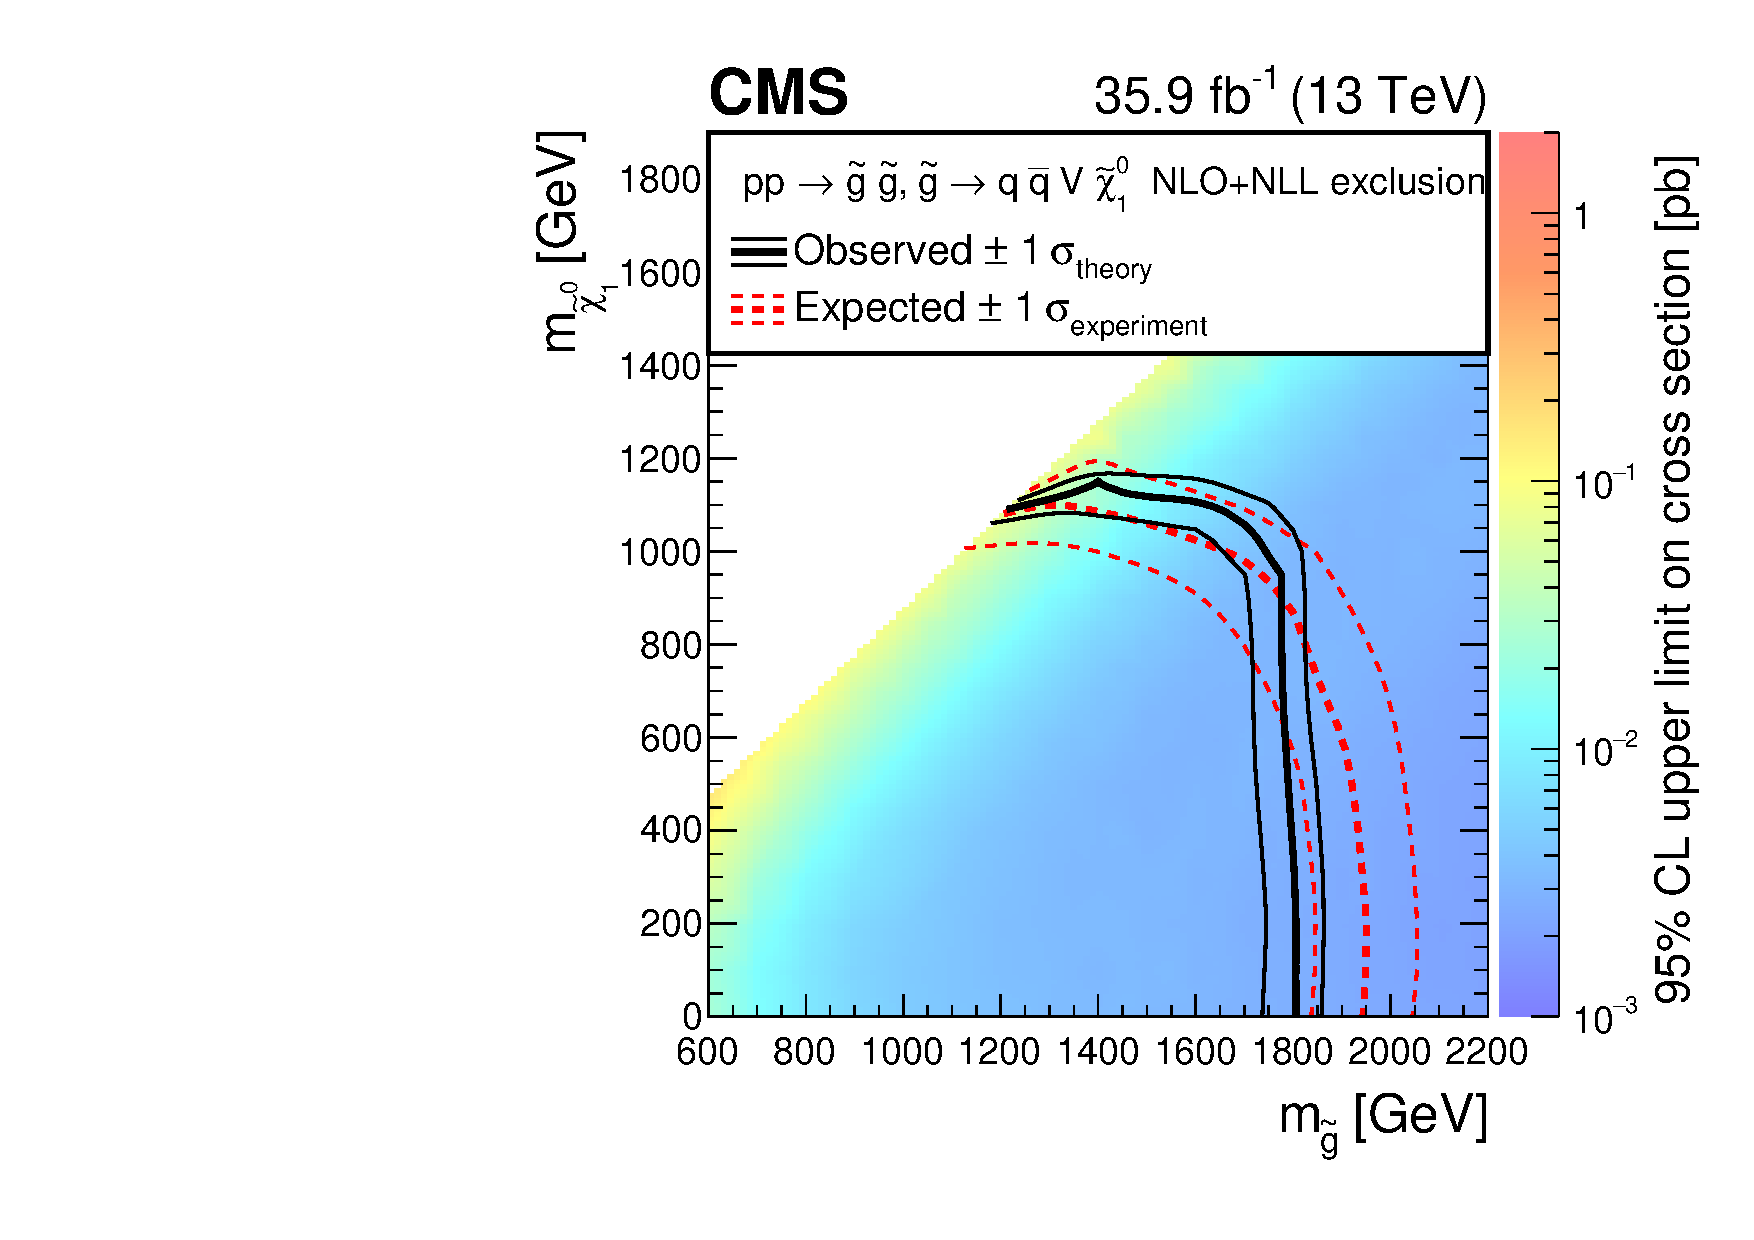
\includegraphics[width=\textwidth]{figs/CMS-SUS-16-033_Figure_012-d.pdf}
\end{subfigure}
%\begin{subfigure}{0.35\textwidth}
%\centering
%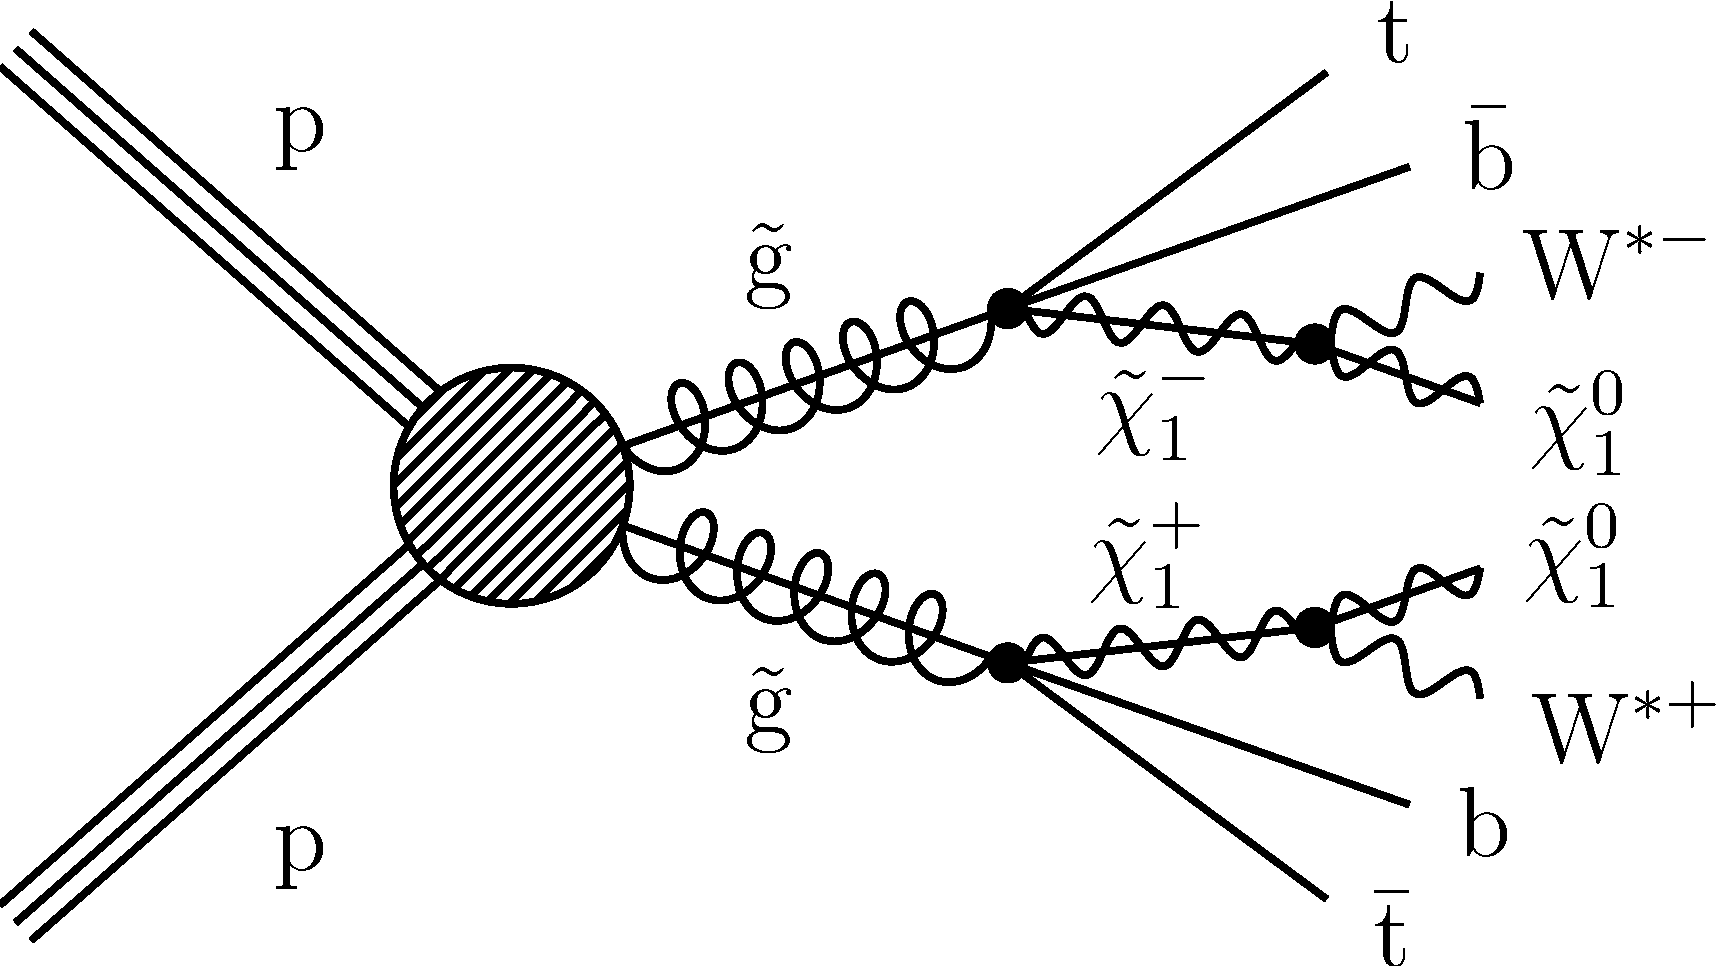
\includegraphics[width=\textwidth]{figs/CMS-SUS-16-033_Figure_001-b.pdf}  
%\end{subfigure}
%\begin{subfigure}{0.45\textwidth}
%\centering
%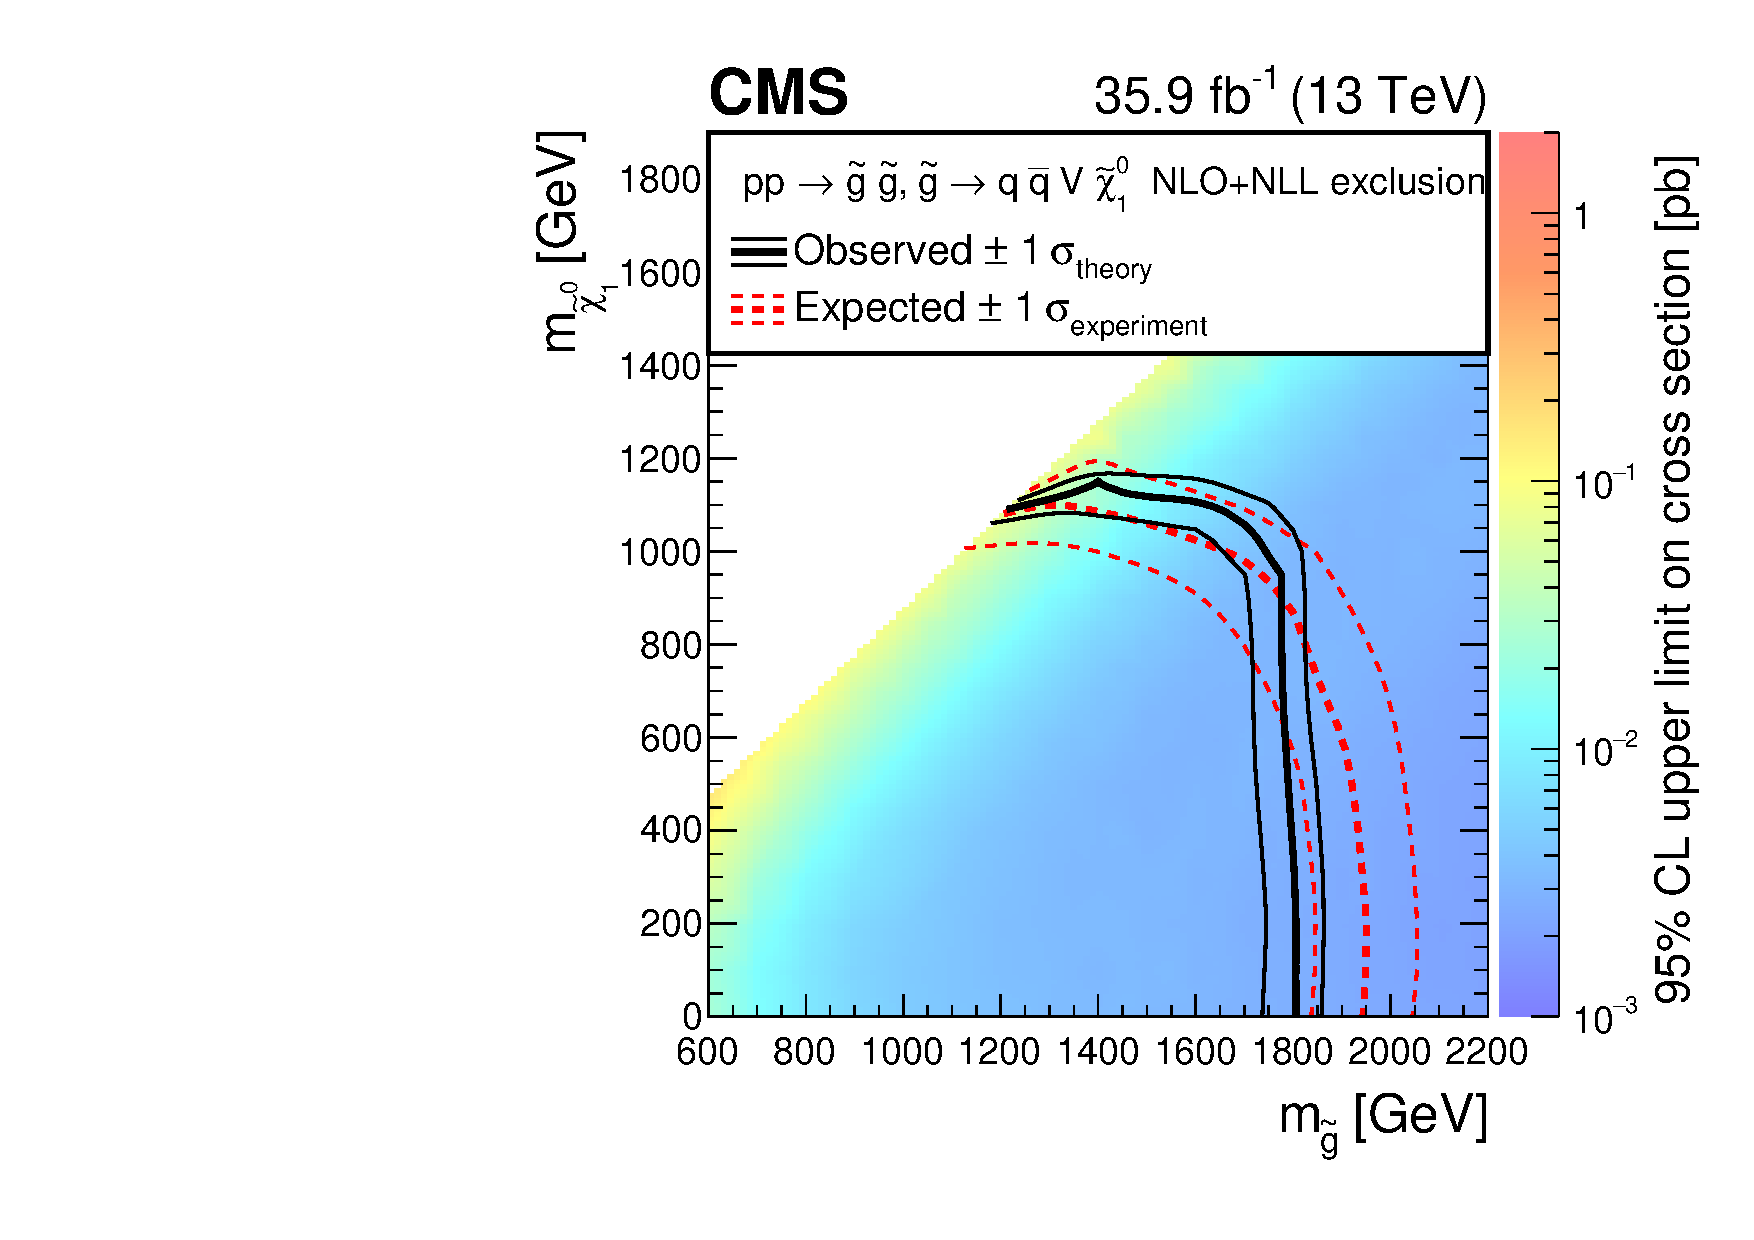
\includegraphics[width=\textwidth]{figs/CMS-SUS-16-033_Figure_012-d.pdf}
%\end{subfigure}
\begin{subfigure}{0.45\textwidth}
\centering
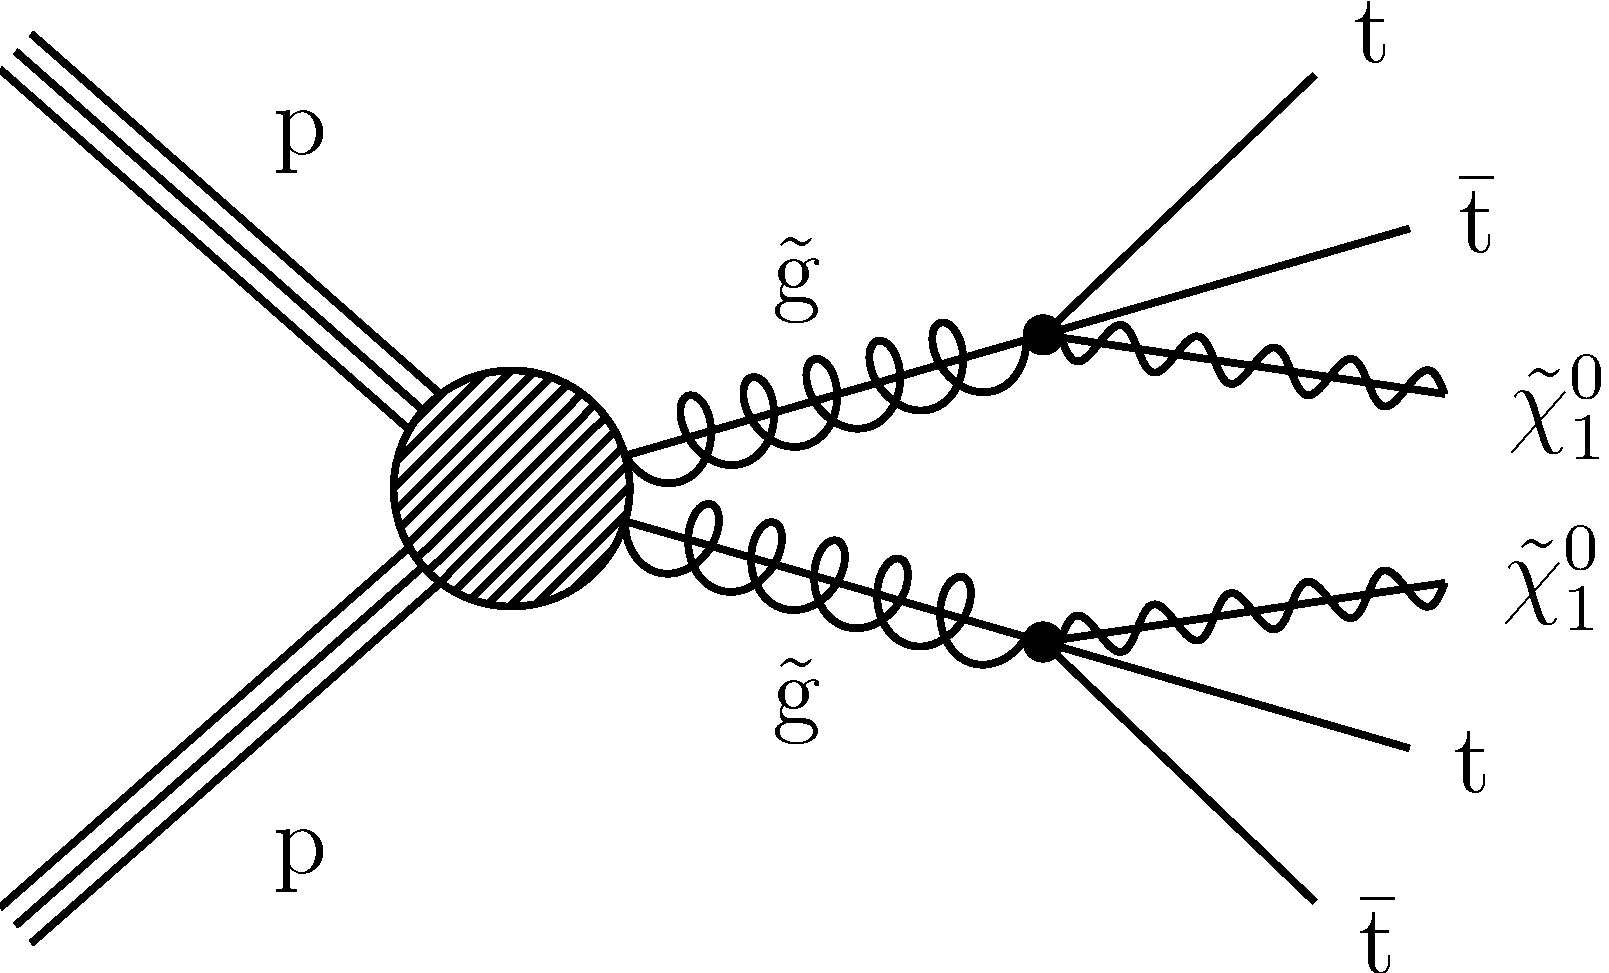
\includegraphics[width=0.7\textwidth]{figs/CMS-SUS-16-033_Figure_001-a.pdf}  
\end{subfigure}
\begin{subfigure}{0.45\textwidth}
\centering
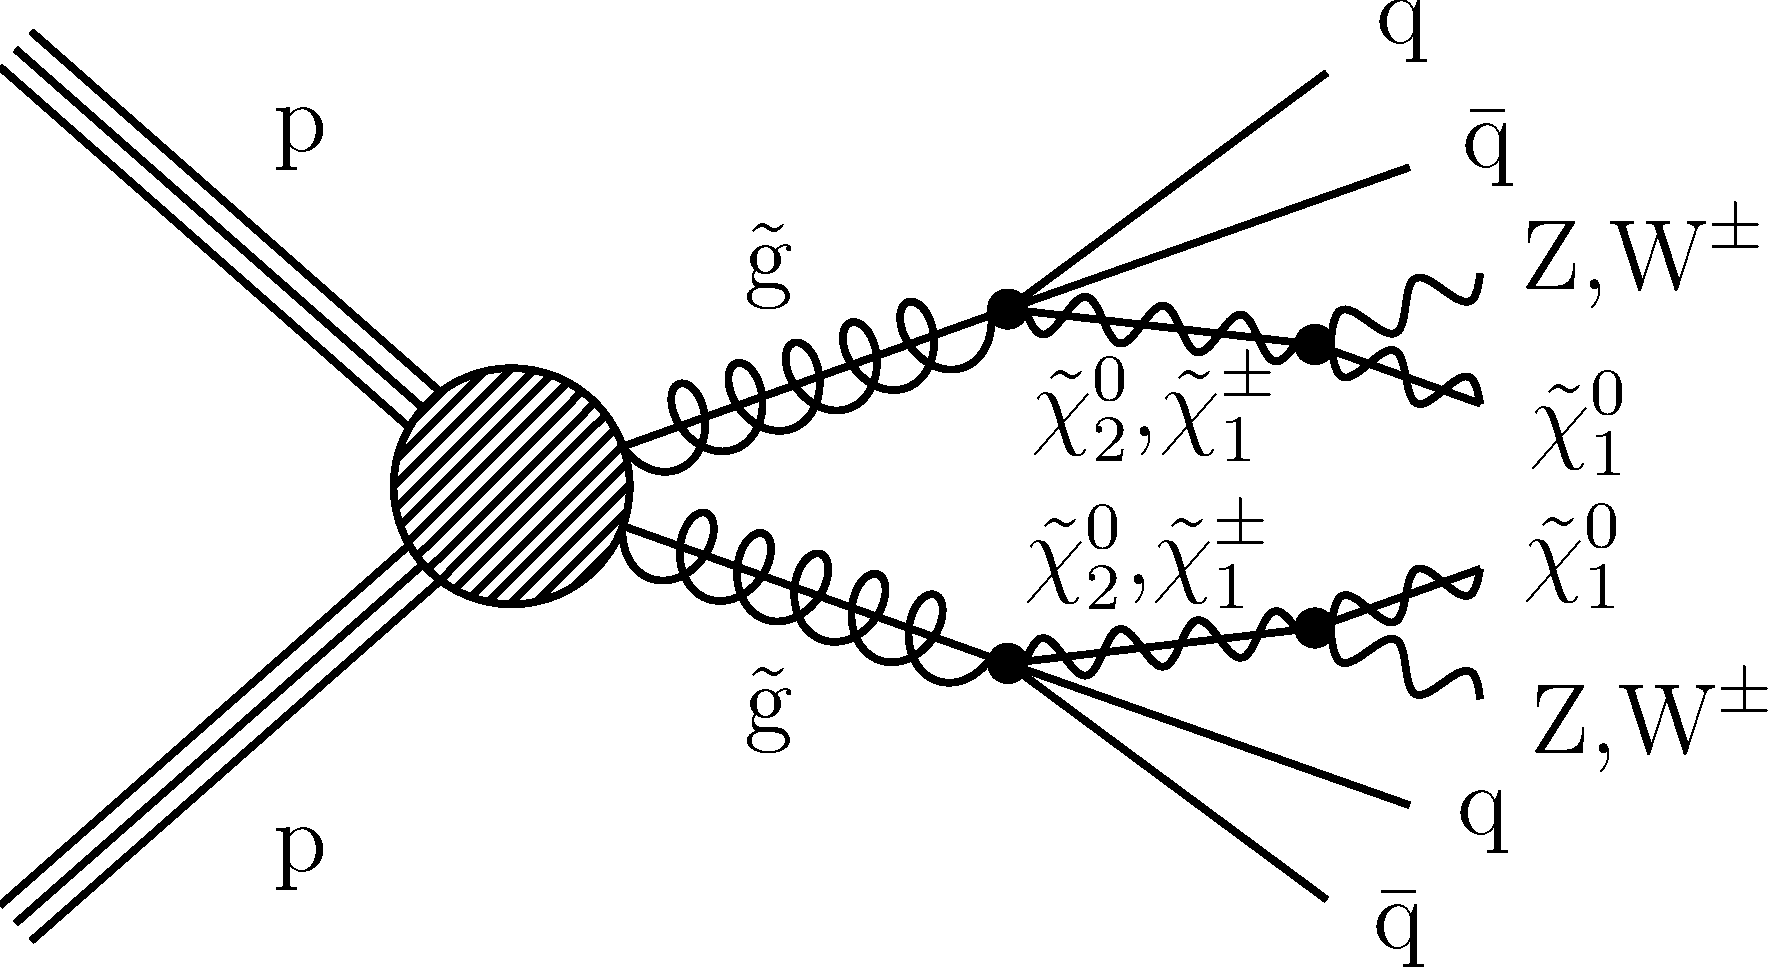
\includegraphics[width=0.75\textwidth]{figs/CMS-SUS-16-033_Figure_001-c.pdf}
\end{subfigure}
\caption{Previous results for searches of gluino-mediated supersymmetry for two gluino decay models: T1tttt (left) and T1qqqqVV (right). The excluded regions are to the lower left. \cite{CMS-SUS-16-033}}
\label{fig:oldlimits}
\end{figure} 
